\documentclass{standalone}
\usepackage{tikz}
\usetikzlibrary{patterns}

%: === TIPOGRAFÍA === (((
\usepackage{fontspec}
\setmainfont[
  BoldFont       = bodonibi,
	ItalicFont     = Century modern italic2.ttf,
	BoldItalicFont = bodonibi,
	SmallCapsFont  = lmromancaps10-regular.otf
]{Century_modern.ttf}
\DeclareSymbolFont{italics}{\encodingdefault}{\rmdefault}{m}{it}
\DeclareSymbolFontAlphabet{\mathit}{italics}
\ExplSyntaxOn
\int_step_inline:nnnn { `A } { 1 } { `Z }
 {  \exp_args:Nf \DeclareMathSymbol{\char_generate:nn{#1}{11}}{\mathalpha}{italics}{#1} }
\int_step_inline:nnnn { `a } { 1 } { `z } {  \exp_args:Nf \DeclareMathSymbol{\char_generate:nn{#1}{11}}{\mathalpha}{italics}{#1}}
\ExplSyntaxOff
% )))

\begin{document}

\begin{tikzpicture}[>=latex]
	\clip (-4,0) rectangle (6.5,4);
	% \fill [gray!20] (0,0) rectangle (-4cm,4cm);
	\draw (0,0) rectangle (-4,4);
	\node [opacity=0.25] at (-2,2) {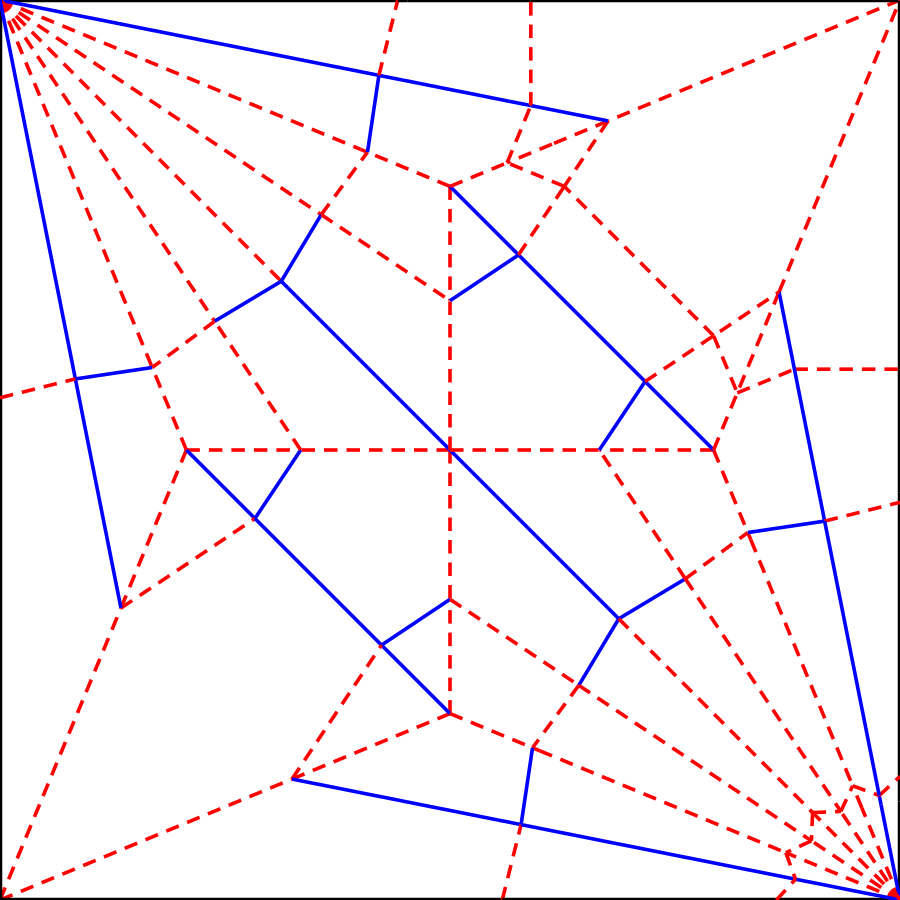
\includegraphics[width = 4cm, height = 4cm]{crane.png}};
	\node at (4.5,2) {
\includegraphics[width = 4cm, height = 4cm]{swan.png}};
	\draw [->, xshift=0.4cm] (0.2,2) to [out=20 , in=160] node [above,midway] {\(T\)} (1.8,2);
	\def\a{1.5*0.88}
	\def\b{0.62*0.88}
	\def\t{238}
	\def\r{0.34}
	\def\s{0.95}
	\def\th{315}
	\draw [dash pattern = on 6pt off 2pt, thick ,red] (0,4)
	 -- (-\a,4-\b)
	 --++ (\t:\r)
	 --++ (\th:\s)
	 -- (-\b,4-\a)
	 -- cycle;
	 \fill [green] (-0.7,2.9) circle (2pt);
	 \fill [blue] (-1,3.45) circle (2pt);
	 \fill [orange] (-1.2,3) circle (2pt);
\end{tikzpicture}

\end{document}
